% !TeX root = these.tex

\chapter{Cadre technologique}


\section{Développement du côté client}
%*****************************Google Web Toolkit***************************
\subsection{Google Web Toolkit (GWT)}

	%************************ Présentation *********************************
\subsubsection{Présentation}
C'est un outil open source permettant de développer des applications web avancée. En utilisant cet outil, nous pouvons développer des applications AJAX en langage Java. 
Le "cross-compiler" gwt traduit l'application java en fichiers JavaScript, qui sont très optimisé (et optionnellement "obscurci" (rendre le code "illisible").
GWT n'est pas "just another library" mais possède ça propre philosophie.

Pour programmer une application web aujourd'hui, il faut maîtriser le Javascript, l'HTML ainsi que le CSS. Le problème principal de ces outils est la compatibilité des navigateurs. En effet, la façon de mettre en forme un site web, n'aurai pas toujours le même rendu sur Internet Explorer, que sur Firefox, Safari, ou encore Chrome ou opera. Il faut prendre en compte aussi, la difficulté d'utilisation de ces outils de manière avancée (utilisation du DOM en HTML, le javascript,…). Le langage Javascript est assez complexe d'utilisation, surtout pour l'écriture de grosse application (c'est d'ailleurs pour ces raisons que beaucoup utilise des librairies / framework javascript plutôt que de tout codé eux même). De plus, le debuggage d'application écrite en javascript est assez fastidieux celui-ci étant un langage interprété. Pour pallier à ces problèmes, GWT à été créé. Il a été élaboré dans le but de répondre à un besoin, et non pas de proposer un "autre libraire". GWT est une vrai boite à outils, et propose des solutions de développement répondant au besoin du programmeur.
% ici je rajouterais qq lignes sur le fait que gwt est énormément utilisé par 
% des société prestigieuse ainsi que google

%************************ Principe de fonctionnement *********************************
\subsubsection{Principe de fonctionnement}
GWT possède un plugin pour Eclipse (et pour d'autre IDE comme NetBeans, JDeveloper,…). Ce plugin, dans sa version Eclipse, permet d'invoquer le compiler GWT, Créer des configurations de "running",… Il s'agit donc d'un outils très puissant qui favorise la facilité. Il se fond parfaitement à l'IDE et est très simple et très pratique d'utilisation.
Le principe de fonctionnement de GWT est de pouvoir créer des applications web basé sur le modèle client/serveur en Java, et de convertir ce langage en javascript. La partie Client de l'application est traduite en javascript, la partie serveur reste en java. Le programme peut être compilé pour un ou plusieurs navigateurs. Ainsi, le projet peut être compilé pour Internet explorer et/ou Firefox, Chrome, etc… Ceci nous garanti une homogénéité de l'application web entre les différents navigateurs. Ces deniers ne chargent uniquement que ce qui les concernes. En plus de ces différents aspects qu'offre GWT, il permet aussi de préciser quelle class prendre en compte pour tel navigateur.

%************************ Mode de fonctionnement *********************************
\subsubsection{Mode de fonctionnement}
Nous distinguons deux types de fonctionnement. Le mode de développement ainsi que le mode de production.
	
\paragraph{Mode de développement}
Le mode de développement consiste à compiler les sources (.class) du projet. Celui-ci n'est pas retranscrit en Javascript mais est directement exécuté en en byte code. Ceci afin de permettre le debuggage de l'application. GWT compile aussi le projet en javascript html et css afin de valider le projet.
Pour pouvoir utiliser le mode de développement, il est nécessaire d'installer au préalable le plugin de développement sur le navigateur. Ce plugin permet de capturer les événements et actions venant du client et de les envoyer vers le serveur.
\paragraph{Mode de production}
Le mode de production quand à lui, correspond au code javascript généré par le compilateur GWT. Le compilateur créer le javascript, HTML et CSS a partir de sources du projet (.class). C'est l'application final tel que nous la connaissons sous forme de ".war". Elle est destiner à être envoyer sur un serveur (Tomcat dans notre cas) et à être utilisée par l'utilisateur final.

%****************************Architecture de GWT******************************
\subsubsection{Architecture GWT}
L'architecture d'un projet GWT se fait sous la forme de client/serveur. Nous distinguons deux types de communication dans l'application.
Client/Client: communication entre les différentes vue de l'application
Client/Serveur: utilisant le protocole RPC 

\paragraph{Évènement}
Afin de pouvoir communiquer et d'envoyer des informations entres les différentes vues de l'application, gwt utilise un système d'envoi "d'event". Celui-ci permet au vue de dialoguer entre elle.
Par exemple, une application gwt peu posséder un header. Celui-ci est statique et n'est pas recharger entre les différentes vues. Lorsqu'on se connecte (login) à l'application, celle-ci peut envoyer les informations de connexion à la vue suivante pour spécifier que nous sommes bien connecté.
Les events sont enregistré auprès de "l'eventbus". Qui se charge d'envoyer les évènements à travers l'application.

\paragraph{Actions}
Les actions ressemble au Event, à l'exception que celle-ci sont envoyer au serveur. Elle permette par exemple de faire des requêtes vers la base de données pour recueillir certaines informations. Pour rester dans le même exemple, lorsqu'un utilisateur se connecte à l'application en spécifiant sont identifiant et son mot de passe, ceux-ci doivent être vérifié dans la base de donnée qui va renvoyer, dans le cas ou l'utilisateur existe, la liste des projets qui lui sont assigné. Cette méthode ce fait à l'aide du protocole JSON/RPC (don nous discuterons dans un autre point). Il existe différent type de RPC (qui sont incompatible entre eux). Les appels se font de manière asynchrone ceci afin de ne pas bloquer le client lors d'un appel de procédure.
	
%***************************** Avantage de GWT****************************
\subsubsection{Avantages}

\paragraph{Facilité d'utilisation}
Le premier avantage que nous citerons est la facilité d'installation et d'utilisation de l'outil. Pas besoin de configuration fastidieuse. Installer Eclipse, Installer le Plugin, et ça fonctionne.
Avec GWT, il devient plus facile d'établir des applications web. Pas besoin de grande connaissance du javascript, nous pouvons coder dans un langage haut niveau.

\paragraph{Debbugage}
Il permet un debuggage rapide du code, celui-ci étant codé en java et non pas en javascript qui est un langage interprété.

\paragraph{Optimisation}
Optimisation du code, obfuscation de celui-ci, compression du JS, mise en cache, séparation du JS en différent fichier,… La question d'optimisation sera le sujet d'un autre point.

\paragraph{prédéfini de composant}
Il propose tout un tas de widget, ainsi, pas besoin de passer des heures a designer un bouton, une boite de dialogue, etc… avec la possibilité de créer ces propres widget.

\paragraph{Code adapter en fonction du navigateur}
Le code java est traduit en code javascript et automatiquement adapté à tout type de navigateur (IE, Firefox, Chrome, mais aussi les navigateur pour appareil mobile)

\paragraph{JSNI (javascript native interface)}
GWT offre la possibilité d'utiliser directement du code javascript. Il est donc tout à fait possible d'utiliser des librairies externes comme Jquery, et de les utiliser dans l'application.

\paragraph{Internationalisation}
Prise en charge de manière native

%**************************** Inconvénient de GWT **************************************
\subsubsection{Inconvénients}
Le principal inconvénient est qu'une fois que le projet atteint un certain avancement, il devient très lourd et très lent de tester son application en mode développement. En effet, la JVM traduit le code java, et est très lente. Il nous faut en moyenne 5 minutes pour charger une page, et nous avons eu frequement des erreurs de type "out of memory". Pour certains type de test, il nous a d'ailleurs été obliger de déployer a chaque fois l'application sur notre serveur tomcat, car la traduction du java vers le javascript étant tellement lente, certaine chose était tout simplement intestable en mode de développement (notement le drag and drop,…). De même lorsque l'application doit charger une grande quantité d'information (grand nombre de carton, professeur,…) la page mais beaucoup de temps à s'ouvrir.
Autre inconvénient et le temps de compilation du logiciel. Celui-ci peut être très fastidieux en fonction des paramètres demandé.
	
Un autre inconvénient est la limitation des widgets fournis de base dans l'application. Pour certaines chose plus avancée nous avons du avoir recourt à des librairie externe, bien que celle-ci ne soit pas aussi performante (comboBox avec CheckBox,…).

%************************* GWT DESIGNER *******************************
\subsection{GWT-Designer}
GWT-Designer est un outils permettant de créer de manière simple les interfaces graphiques. Celle-ci est créer via un fichier xml et est retranscrite en code java par le compilateur. Ce code xml est soit éditable "manuellement" ou peut être créer via une interface de drag and drop ou les composants (widgets) peuvent être sélectionner. L'avantage d'utiliser un tel outils est la bonne pratique que celui-ci apporte, permettant de faire une distinction entre les différentes partie du code.

%************************* GWT PLATEFORM *********************************$
\subsection{GWT - Plateform}

\subsubsection{Présentation}

GWT plateform est un framework basé sur le MVP (model view presenter) et permettant de simplifier la creation de projet GWT. Il favorise les "bonne pratique" lors de la conception d'un logiciel.
	
\subsubsection{Le model View Presenter}
Le MVP se base sur le MVC (model view controler). Celui-ci est un design pattern permettant de donner une manière d'élaborer des interfaces graphique. Il est donc séparé en trois partie, le modèle de donnée, les différentes vues de l'application (ce que vois l'utilisateur: l'interface) et le présenteur (correspondant au controleur du MVC). Dans le model view controler le controleur s'occupe de gérer les évenements. La logique de contenu (Rendering logic) se passe directement entre le modèle et la vue. En MVP, cette logique est géré par le présenteur, ansi, plus rien ne transite entre l'interface et le modèle de façon direct, mais est soumise au contrôle du présenteur. (peut être un peu mieux expliquer le truc,…)

%*************************** LIBRAIRIE EXTERNE GWT **************************
\subsection{Libraire externe}
Pour certaines choses plus avancée nous avons du nous tourner vers des librairies externe. 
\subsubsection{GWT-dnd}
Nous avons utiliser GWT-dnd qui comme son nom l'indique nous a permis
d'implémenter le drag and drop sur les cartons. Le drag and drop fournis par
cette librairie nous permet de capturer les évenements de la sourir mais aussi les évenements touch (et donc, de garder la possibilité qu'offre GWT d'être utiliser sur des appareils mobile). Ce qui est non négligable à l'heure actuelle ou les smartphones et tablettes on une place prépondérante pour le consomateurs ainsi que pour les entreprises. Cette librairie permet de rendre dragable n'importe quel widget, ou un ensemble de ceux-ci. Afin de pouvoir réaliser cette opération, il est nécéssaire de créer un "dragcontroler" et d'y ajouter toutes les parties, ou chaque widget que nous voulons rendre dragable. Il est possible aussi d'enregistrer (meilleur mot pour ça?) au près de ce dragcontroler, un ou plusieur dropcontroler (targer) ou peut être déposer ce qui a été rendu draggable.

\subsubsection{Smart-GWT}
Smart-GWT est un wrapper de la librairie javascript SmartClient. Elle propose un grand nombre de wiget qui peuvent venir s'ajouter à ceux fournis par GWT. Puisque Smart-GWT n'est qu'un wrapper de la smartClient, elle ne respecte pas l'idée de base de GWT étant que le code soit écrit totalement en java et ensuite traduit en javascript. Nous avons pu noté que les widgets proposer par cette librairie ne sont pas aussi réactif que ceux proposer par GWT, ou encore, ceux que nous avons créer nous même.
Ces deux libraires on été spécialement concue pour être utilisée avec GWT. Il ne s'agit pas de librairie javascript comme Jquery, mais bien de librairie orienté GWT. Elles sont fournies sous forme de .jar, il faut changer le fichier (xml) de configuration du projet et y rajouter le chemin pour y accéder.


%\subsection{Serveur Linux}
%SERVEUR LINUX (Debian 64bits)
%Afin de pouvoir tester notre application, nous disposons d'un serveur tomcat tournant sur une machine %linux. L'application (sous forme de ".WAR" (en comparaison au ".jar", le "W" signifiant web)) est %l'application final possédant le code javascript (et non plus du code java comme en mode de %développement).

\subsection{Les langages web}
L'évolution des navigateurs, des langages web et des possibilités que ceux-ci permette, l'évolution de la société visant à s'orienté de plus en plus vers le cloud computing nous montre l'utilité d'utiliser ces langages dans leur dernière normes. Afin de proposer une application web interactive, nous nous sommes orienté sur ces derniers langage web, même si nous n'utilisons pas tout l'étendu de ce qu'ils proposent.

\subsubsection{HTML5}
GWT nous permet l'utilisation du HTML5. l'arriver du HTML5 permet d'accroitre les performances d'une application web, en proposant des fonctionnalité plus avancées tel que l'utilisation de canvas, de balise audio ou video. Une autre fonctionnalité est l'utilisation d'un local storage, permettant de stocker une grande quantité de donnée.
\subsubsection{CSS3}
Le design général de l'application a été basé sur cette dernière norme. Il est donc nécessaire d'avoir un navigateur à jour pour pouvoir profiter de l'avantage qu'offre cette norme.

\subsubsection{JavaScript}
Même si le code javaScript est généré par le compilateur de GWT, elle est un élément essentiel de l'application. 
 
\subsection{Local Storage (LS)}
L'apparition du local storage avec le HTML5 ouvre une porte en plus au développeur d'application web. Ce dernier permet de stocker une grande quantité de données coté client. Pour bien comprendre le choix de l'utilisation de cette technologie, nous allons le comparer avec le cookie.

\subsubsection{Local Storage vs Cookies}

LOCAL STORAGE
Capacité de stockage : 5MB
Utilisation de la bande passante: Aucune, tout est stocker chez le client)
Performance: Data mise en cache du navigateur
contraintes: aucune
rapidité: rapide (charge les données de la cache au démarrage)

COOKIE
Capacité de stockage: 80KB (4KB/cookie 20cookies/domaine)
Utilisation de la BP: Envoi des données a chaque requete vers le domaine
Performance: Data envoyé répétitivement vers le domaine
contraintes: 300 cookies maximum
rapidité: plus lente (serveur vérifie si le cookie existe)

Tout comme les cookies, les informations contenu dans le local storage ne peuvent pas contenir d'information sensible (numéro de carte de crédit, etc...). Nous ne nous sommes pas attarder sur ce point car les informations contenu dans le local storage (information sur les activités) ne sont pas utile pour les Hackers. Pas besoin de crypter le nom d'un professeur. 

L'utilisation du local storage permet, comme les cookies, de partager les données entre les différents onglet du navigateur. Nous aurions pu nous orienté vers une solution plus simple, comme enregistrer les informations de la partie cliente dans des tableaux ou listes, mais les informations ne serait plus partager entre les différents onglet et fenêtre du navigateur, ce qui limiterais de manière drastique l'utilisation du programme. Le local storage à donc bon nombre d'avantage et l'utilisation et la mise en place de celui-ci, bien qu'étant une partie fastidieuse, était pour nous nécessaire au bon développement de l'application ainsi qu'a sont développement futur.

\subsubsection{Principe}
Le principe de ce local storage est donc de fournir un moyen de stocker et d'accéder au données de manière rapide tout en limitant le trafic entre le client et le serveur. Nous ne rentrerons pas dans la structure de celui-ci, ce point faisant partie d'un autre chapitre. Les informations sont mise dans en cache et peuvent être supprimer à tout moment par l'utilisateur.
\subsubsection{Utilisation dans notre application}
Lors de chaque modification (comme le placement d'un carton), nous enregistrons ces changements dans le LS ainsi que dans la base de données de manière asynchrone afin de permettre une grande rapidité de l'application. Dans l'hypothèse ou la base de données ne serait plus accessible (ex: perte de connexion) nous avons implémenté une fonctionnalité\footnote{version alpha} permettant de synchroniser l'état du local storage avec la base de données lors d'un retour de connexion.\\
\\
Actuellement, une connexion internet est requise lors d'un rechargement de la page afin de se mettre à jour, ceci est indispensable pour offrir une synchronisation cohérente. Cependant une fonctionnalité, en Alpha actuellement, permet, si l'option est activé ou si la bdd n'est pas accessible, de fonctionner sans cette dernière, et lors de la récupération de la connexion, les données sont alors synchronisé.



\section{Développement du côté serveur}

\subsection{Java EE}

% A retravailler
La plateforme Java entreprise (Java EE) est un ensemble de spécifications portée par un consortium de sociétés internationales qui permettent ensemble des solutions pour le développement, le déploiement, et de la gestion des applications d'entreprises multi-niveaux, basées sur des composants.

\begin{figure}[!h]
    \center
   	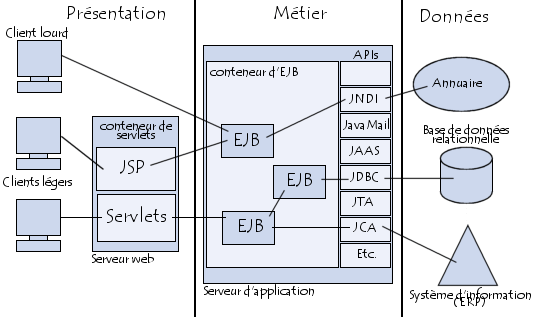
\includegraphics[scale=0.65]{architecture_JEE.png}
   	\caption{Diagramme issu de\url{architecture_JEE.png}}
    \label{reference1}
\end{figure}

Et dans la figure  \ref{reference1}\footnote{Diagramme issu de \url{}}
** image**
Construit sur la plateforme de Java 2 édition standard (Java SE), la plateforme Java EE ajoute les possibilités nécessaires pour fournir une plateforme complète, stable, sécurisée, et rapide de Java au niveau entreprise. 
Dans la mesure où J2EE s'appuie entièrement sur le Java, il bénéficie des avantages et inconvénients de ce langage, en particulier une bonne portabilité et une maintenabilité du code.\\
\newline
\indent
L'ensemble de l'infrastructure d'execution JavaEE est donc constitué de services (API) et spécifications tel que:
HTTP et HTTPS
Java Transaction API (JTA)
Remote Method Invocation/Internet Inter-ORB Protocol (RMI/IIOP)
Java Interface Definition Language (Java IDL)
Java DataBase Connectivity (JDBC)
Java Message Service (JMS)
Java Naming and Directory Interface (JNDI)
API JavaMail et JAF (JavaBeans Activation Framework)
Java API for XML Processing (JAXP)
Java EE Connector Architecture
Gestionnaires de ressources
Entreprise Java Beans (EJB)
Java Server Pages (JSP)
Servlet
Java API for XML Web Services (JAX-WS, anciennement JAX-RPC)
SOAP with Attachments API for Java (SAAJ)
Java API for XML Registries (JAXR)

Dans le cadre de notre application, seule une sous partie de ces composants nous ont été utile, tel que, notemment, les servelets, les JSP, JavaMail ou encore Jdbc avec hibernate, tel que décrit dans le point suivant.

De plus, l'architecture J2EE repose sur des composants distincts, interchangeables et distribués, ce qui signifie notamment :

qu'il est simple d'étendre l'architecture ;
qu'un système reposant sur J2EE peut posséder des mécanismes de haute-disponibilité, afin de garantir une bonne qualité de service ;
que la maintenabilité des applications est facilitée.

Pour interagir avec notre solveur d'une part, de la base de données d'autre part, et par


%% ==== avantages
java EE vs php vs .net vs python

%% === apprentissage
Ce fut nouveau mais xxx
Ca nous à permit d'apprender les outils et les techniques les plus recherchée actuelement 

\subsection{Hibernate}

Pour pouvoir communiquer avec notre base de donnée à partir de notre code java, on a commencé avec jdbc\footnote{Java Database connectivity} mais cela n'était pas suffisant et on s'est tourné ver Hibernate.

Hibernate est un framework libre, appellé framework de  "mapping objet-relationnel" ou encore de "persistance objet des données" (voir Figure \ref{reference2}). 
\begin{figure}[!h]
    \center
   	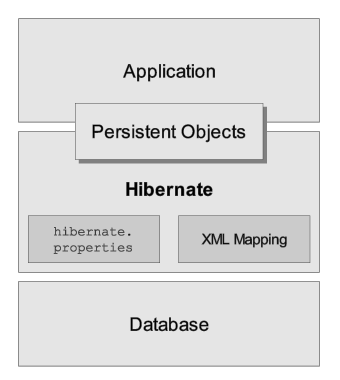
\includegraphics[scale=0.65]{schema_hibernate.png}
   	\caption{Diagramme issu de\url{}}
    \label{reference2}
\end{figure}
Ca permet donc à la couche applicative de notre programme de traiter les données vennant de la base de donnée comme des objects donc le contenu reste en mémoire même après la fin d'exécution du programme. D'où persistance objet des données. Le lien entre les classes exposées et la source physique des données (dans notre cas une base de données *relationnelle*) est définie par un fichier xml. D'où mapping objet-relationnel.
Cela nous à permit de gérer notre base de données, comme le reste de l'application en orienté objet, et même si son apprentissage ne fut pas des plus aisée, la gestion générale du code s'en est retrouvé grandement amélioré.

Un autre avantage recherché par cette solution, est que son indépendance à la base de donnée le rend ultra portable, et, sans aucune modification du code, notre application peu tourner sur 221\footnote{http://developers.sun.com/product/jdbc/drivers} base de données différente.  Notre application, après avoir configuré ses crédential dans le fichier de configuration d'Hibernate, se chargera de créer l'entièretée des tables et la structure de la base de donnée.

Théoriquement il aurait donc été possible d'envoyer directement un objet "hibernate" (représentant par exemple une table de notre bdd), à gwt, donc à l'utilisateur, malheureusement le monde n'est pas parfait, et comme stipulé dans la doc GWT\footnote{https://developers.google.com/web-toolkit/articles/using\_gwt\_with\_hibernate},
une SerializationException est levée à chaque fois un type transférée sur RPC n'est pas «sérialisable». La définition de la sérialisibilité signifie ici que le mécanisme RPC GWT sait comment sérialiser et désérialiser le type de bytecode au format JSON et vice-versa.
Le problème vient du fait qu'Hibernate modifie les objects afin de les rendre persistant (pour être exact, c'est la librairie javassist qui se charge de réécrire le bytecode de ces objects pour les rendre persistant). Au moment du transfer de l'object, une serialisation est tantée, mais n'étant pas le même (car modifé par javassist), il ne peut être sérialisé par RPC-GWTP.
Il a fallut donc rajouter des classes de type DTO\footnote{Data Transfer Object}, qui, eu sérialisable ont pu servir de communiquation entre la partie cliente et serveur.

Hibernate possedant sont propre language de requète HQL \footnote{Hibernate Query Language}, d'apparence similaire au SQL, mais pleinement orienté Object et comprenant des notions comme l'inheritance ou le polymorphisme\footnote{https://docs.jboss.org/hibernate/orm/3.3/reference/en/html/queryhql.html}.  Mais ca nous à bien fais chier (xx), et on a pas su en tirer pleinement avantage.




\section{Outils côté client/serveur}





